\documentclass[onecolumn,10pt]{article}
\usepackage[english]{babel}
\usepackage{times}
\usepackage{graphicx}
\usepackage{amssymb,amsmath}
\usepackage{dsfont}
\usepackage{hyperref}
\usepackage {graphicx}
\usepackage {xspace}
\usepackage{mathtools}
\usepackage[dvipsnames]{xcolor}
\usepackage{enumitem}

%\input ../../lectures/notation.tex

\usepackage[margin=0.6in,foot=0.25in,nohead]{geometry}
\newcommand{\Rx}[1]{\mathds{R}^{#1}}
\newcommand{\ie}{\emph{i.e.} \xspace}
\newcommand{\eg}{\emph{e.g.} \xspace}
\newcommand{\etc}{\emph{etc.} \xspace}

\def\captionfonts{{\em}}
\makeatletter  % Allow the use of @ in command names
\setlength{\abovecaptionskip}{0.3ex plus 0.3ex minus 0.3ex}
\setlength{\belowcaptionskip}{0.3ex plus 0.3ex minus 0.3ex} 
\long\def\@makecaption#1#2{%
  \vskip\abovecaptionskip
  \sbox\@tempboxa{{\captionfonts #1: #2}}%
  \ifdim \wd\@tempboxa >\hsize
    {\captionfonts #1: #2\par}
  \else
    \hbox to\hsize{\hfil\box\@tempboxa\hfil}%
  \fi
  \vskip\belowcaptionskip}

\renewcommand\section{\@startsection{section}{1}{\z@}%
                       {-1.8ex \@plus -0.8ex \@minus -0.8ex}%
                       {1ex \@plus 0.4ex \@minus 0.4ex}%
                       {\normalfont\large\bfseries\boldmath
                        \rightskip=\z@ \@plus 8em\pretolerance=10000 }}
\renewcommand\subsection{\@startsection{subsection}{2}{\z@}%
                       {-1.0ex \@plus -0.6ex \@minus -0.6ex}%
                       {1.0ex \@plus 0.3ex \@minus 0.3ex}%
                       {\normalfont\normalsize\bfseries\boldmath
                        \rightskip=\z@ \@plus 8em\pretolerance=10000 }}

\makeatother   % Cancel the effect of \makeatletter


\setlength{\parindent}{0in}
\setlength{\parskip}{1.5ex}

%\long\def\solution#1{\textit{Solution:}\\
%\begin{tabular}{@{\hspace{1ex}}|@{\hspace{1ex}}p{6in}}
%{\begin{minipage}{\linewidth}#1\end{minipage}} \end{tabular}}

%\long\def\solution#1{#1}
\long\def\solution#1{}


%%% for tracking points per question
\usepackage{pgfkeys}
\pgfkeys{
 /points array/.is family, /points array,
 .unknown/.style = {\pgfkeyscurrentname/.initial = #1},
}

\newcommand\questionhaspoints[1]{\pgfkeys{/points array, #1}}
\newcommand\getquestionpoints[1]{\pgfkeysvalueof{/points array/#1}}

% for code formatting
\usepackage{listings,color}
\definecolor{verbgray}{gray}{0.9}
\lstnewenvironment{code}{%
  \lstset{backgroundcolor=\color{verbgray},
  frame=single,
  framerule=0pt,
  language=bash,
  basicstyle=\ttfamily,
  columns=fullflexible}}{}

\begin{document}

%Title here
\vspace{0mm}
\textbf{\large ROB 498/599 3D Robot Perception: HW1 Writeup Template}\\
\textbf{Name:} Jinjia Guo\\
\textbf{Uniqid:} jinjaguo \\
\textbf{Email:} jinjaguo@umich.edu \\

\vspace*{1mm}
\hrule
\vspace*{1mm}

\noindent
\vspace{1mm}

\noindent
%\textbf{Data:} You need to download the supplemental data to complete this assignment.  All paths in the assignment assume the data is off the local directory.  The download has data and code; it is named \texttt{hw1.zip}.  \vspace{1mm}


\newcounter{problemnumber}
\setcounter{problemnumber}{0}

\questionhaspoints{0=0,1=20,2=20,3=20,4=10,5=20,6=10}


\noindent\textbf{Instructions: } 
Each bullet point in this template contains the prompt for what information should be included in the write up. Replace the bullet point with your own answer to the question/prompt described in the bullet point. Finally, submit a \texttt{.zip} file containing this write-up and a folder \texttt{scripts} with all the python scripts on Canvas. 

\addtocounter{problemnumber}{1}
\noindent\textbf{Problem \arabic{problemnumber}}: Camera Calibration

 i. In this paragraph, briefly describe the camera calibration process as implemented in your code. How did you obtain your projection matrix? How did you verify it was correct? If you were provided with a different pair of images, how would you obtain projection matrices for the new cameras? In equation \ref{eq:projection_matrix}, report the projection matrix you obtained from your code to 4 significant figures.


\begin{align}
M=\begin{bmatrix}
0.4583& -0.2947& -0.01395&  0.004025\\
-0.05086& -0.05458&  -0.5411& -0.05238\\
0.1090&  0.1783& -0.04427&  0.5968\\
\end{bmatrix}
\label{eq:projection_matrix}
\end{align}

\textbf{Answer:}  

We follow the direct linear transformation (DLT) method to calculate the projection matrix.
The function {\tt  calculate\_projection(pts2d, pts3d} calculates the $3×4$ projection matrix M using a set of corresponding 2D image points and 3D world points.

First, a system of linear equations can be constructed between the 3D points and their 2D projection points in homogeneous coordinates. Since the last element of the M matrix is $1$, we can solve M by constructing 11 equations.

Here we use SVD to solve the $AX = 0$ problem. Since $AX=0$ is an overdetermined equation, there is usually no non-zero solution. By decomposing A with SVD, we find the right singular vector corresponding to the minimum singular value, which is the solution with the minimum norm. In this way, we get an optimal solution with the minimum error and satisfying the unit norm constraint. It is worth noting that the coordinates of the input calculation should be homogeneous coordinates.

Finally, the matrix is normalized.

For the verification of the Projection Matrix. we compare the reprojected points to the given 2D points. The reprojection error is computed as the mean Euclidean distance between the actual and projected 2D points.

If a different pair of images were provided, the same DLT-based approach would be used. Or we can get the transformation matrix between two cameras, then calculate the camera calibration matrix.

\hrule

ii. In this paragraph, describe your reprojection error results. What does this error represent? What units is it in? If you were provided with a different pair of images and had to recreate this process, how would you validate that your re-projection error was okay? Report the reprojection error of your obtained projection matrix in equation \eqref{eq:reprojection_error} to 6 significant figures.


\begin{equation}
errror_{reprojection}=0.00222745 \label{eq:reprojection_error}
\end{equation}

\textbf{Answer:}  

The reprojection error calculated in the code represents the average Euclidean distance between the actual 2D image point and the projected 2D point obtained using the estimated projection matrix. The reprojection error is in pixels because it measures the difference between coordinates in image space.

If we have a pair of different images, we can evaluate it like this:

1. We can use the calculated matrix to project the 3D points onto the image and overlay them on the original image, which can intuitively estimate the difference.

2. If we have multiple sets of 2D-3D corresponding points, if the error does not change much, then it proves that there is no problem

\hrule

\noindent\textbf{Sparse 3D Reconstruction}


\addtocounter{problemnumber}{1}
\noindent\textbf{Problem \arabic{problemnumber}}:  Estimation of Fundamental Matrix

i. Briefly discuss the fundamental matrix - what does it actually represent, and how did you obtain it? Report your obtained fundamental matrix to 4 significant figures below in equation \ref{eq:fundamental_matrix}.

\begin{align}
F = \begin{bmatrix}
\multicolumn{1}{c}{3.5648 \times 10^{-9}} & \multicolumn{1}{c}{-5.9210 \times 10^{-8}} & \multicolumn{1}{c}{-1.6500 \times 10^{-5}} \\ 
\multicolumn{1}{c}{-1.3080 \times 10^{-7}} & \multicolumn{1}{c}{-1.3110 \times 10^{-9}} & \multicolumn{1}{c}{1.1240 \times 10^{-3}} \\ 
\multicolumn{1}{c}{3.0470 \times 10^{-5}}  & \multicolumn{1}{c}{-1.0800 \times 10^{-9}} & \multicolumn{1}{c}{-4.1650 \times 10^{-3}} \\ 
\end{bmatrix}
\label{eq:fundamental_matrix}
\end{align}


In a stereo setup, the fundamental matrix $F$ encapsulates the intrinsic geometric relationship between two images taken from different viewpoints.

For epipolar constraint, we have: $p_2^T F p_1 = 0$, where $p_1$, $p_2$ are the homogeneous coordinates $(x,y,1)$. Geometrically, this expresses that a point in one image lies on the “epipolar line” corresponding to the matching point in the other image. The F matrix contains the spatial geometric relationship between the two images of the stereo pair when shooting (external parameters) and the camera calibration parameters (intrinsic parameters), including rotation, displacement, image principal point coordinates, and focal length.

We use 8‐point algorithm to get it:
According to the epipolar constraint, the following relationship holds:
\begin{equation}
    p_2^T F p_1 = 0
\end{equation}

which \( p_2 = [x'_i, y'_i, 1]^T \) and \( p_1 = [x_i, y_i, 1]^T \) are 3-D points in 3D space. \( P \) is the homogeneous coordinate of the image projected onto the camera planes of \( O_r \) and \( O_l \), respectively, and the quantities involved are known. \( F \) is the basic matrix. Substituting in:
\begin{equation}
    \begin{bmatrix} x'_i & y'_i & 1 \end{bmatrix}
    \begin{bmatrix}
        f_{11} & f_{12} & f_{13} \\
        f_{21} & f_{22} & f_{23} \\
        f_{31} & f_{32} & f_{33}
    \end{bmatrix}
    \begin{bmatrix} x_i \\ y_i \\ 1 \end{bmatrix} = 0
\end{equation}

so we have:
\begin{equation}
    \begin{bmatrix}
        x_i x'_i & x_i y'_i & x_i & y_i x'_i & y_i y'_i & y_i & x'_i & y'_i & 1
    \end{bmatrix}
    \begin{bmatrix}
        f_{11} \\ f_{21} \\ f_{31} \\ f_{12} \\ f_{22} \\ f_{32} \\ f_{13} \\ f_{23} \\ f_{33}
    \end{bmatrix} = 0
\end{equation}

which we have:
\begin{equation}
    Ax = 0
\end{equation}
We can use svd to get $F$, where we constrain the last element to $1$.But since $rank(F) = 2$, after getting the above $F$, we can perform $rank2$ approximation to get the final $F$.

\hrule

\begin{figure}[h]
  \centering
  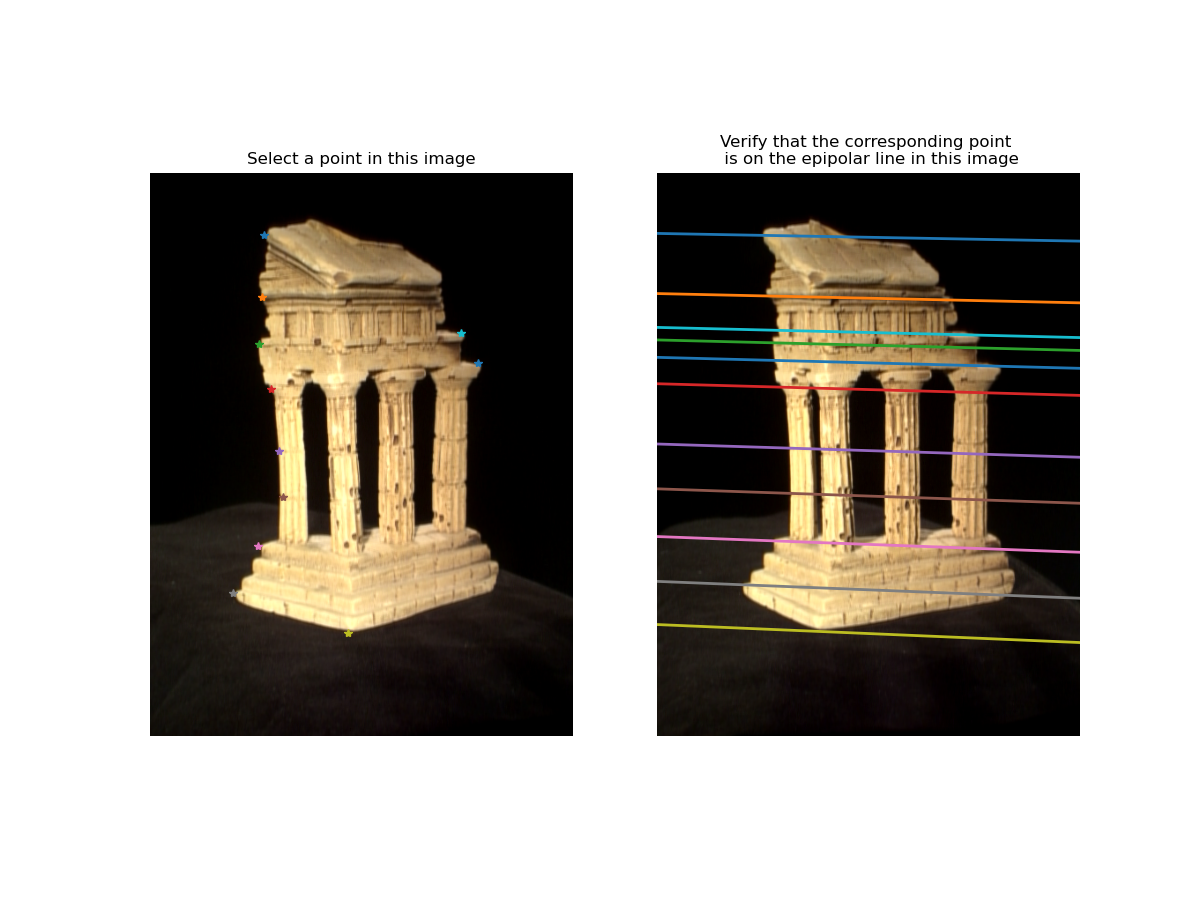
\includegraphics[width=0.66\textwidth]{media/Epipolar line.png}
  \caption{Sample image for GUI output for epipolar lines}
  \label{fig:epipolar lines}
\end{figure}

ii. Discuss how you validated your fundamental matrix. Replace the image in figure \ref{fig:epipolar lines} with a screenshot of your{\tt  epipolar\_lines\_GUI\_tool} results containing at least 6 selected points and reference it here. Were all of the points equally accurate? How did you verify that the drawn epipolar lines were correct? What sources of error exist that may cause these epipolar lines to not be correct?

Epipolar constraint: The most basic check is the epipolar constraint: for corresponding points m and m' in two images, $m'^T F m = 0$. This should hold for all corresponding pairs of points. We can compute this value for many point correspondences and check if they are close to zero. Smaller values indicate better compliance with the epipolar constraint.

Or we can visualize the epipolar lines. For a point $m$ in one image, the corresponding epipolar line in the other image will show up. We can draw these lines and visually check if they are close to the corresponding point $m'$

The points are not very accurate, considering the following factors:

1. Noise in the image will affect the exact location of the detected features

2. Points that are visible in one image but occluded in the other will also lead to incorrect correspondences

3. The precision of the calculation, we use more than one approximation here, which will lead to some errors

\hrule
\addtocounter{problemnumber}{1}
\noindent\textbf{Problem \arabic{problemnumber}}:  Find Epipolar Correspondences

i. Discuss the process for finding correspondances between the two images. What function did you use for your similarity? How did it work? Did you experiment with any other similarity functions, or experiment with any of the parameters (patch size, etc.) of your final function? If so, report on what you tried, and what made you choose your final submitted function.

1. For each point in the first image (pts1), you calculate the corresponding epipolar line in the second image using the fundamental matrix $F: l = F m$, where m is the homogeneous representation of the point.

2. Then use a template matching approach.  A small window (patch) around the point in the first image is used as a template.

3. Using the Sum of Squared Differences (SSD) as your similarity measure: $cost = np.sum((candidate - template) ** 2)$.  This calculates the sum of the squared differences between the pixel values of the template and the candidate patch along the epipolar line. A lower SSD indicates higher similarity.

4. The point along the epipolar line that minimizes the SSD is chosen as the corresponding point in the second image.


I tried using Manhattan distance as the dissimilarity metric, but it didn’t perform as well as SSD.
\hrule
ii. Replace the image in figure \ref{fig:epipolar_corresp} with a screenshot of your {\tt epipolar\_correspondences\_GUI\_tool} results containing at least 6 selected points and reference here. Which correspondences in your image had the best and worst results? What sources of error exist for your correspondance determination process, and how might they be address going forward?

The points at the top of the image are all very good, but the more complex points at the bottom are not so good.

Featureless areas/repeating textures: In areas with little texture or repeated patterns, the similarity metric may not be able to find unique matches
Image noise can affect the accuracy of feature localization and the calculation of similarity metrics. Preprocessing steps such as image smoothing or denoising may help

We can consider preprocessing, image denoising and dedistortion to improve the quality of the input image and bring better matching results, such as Gaussian filtering.
\hrule
\begin{figure}
  \centering
  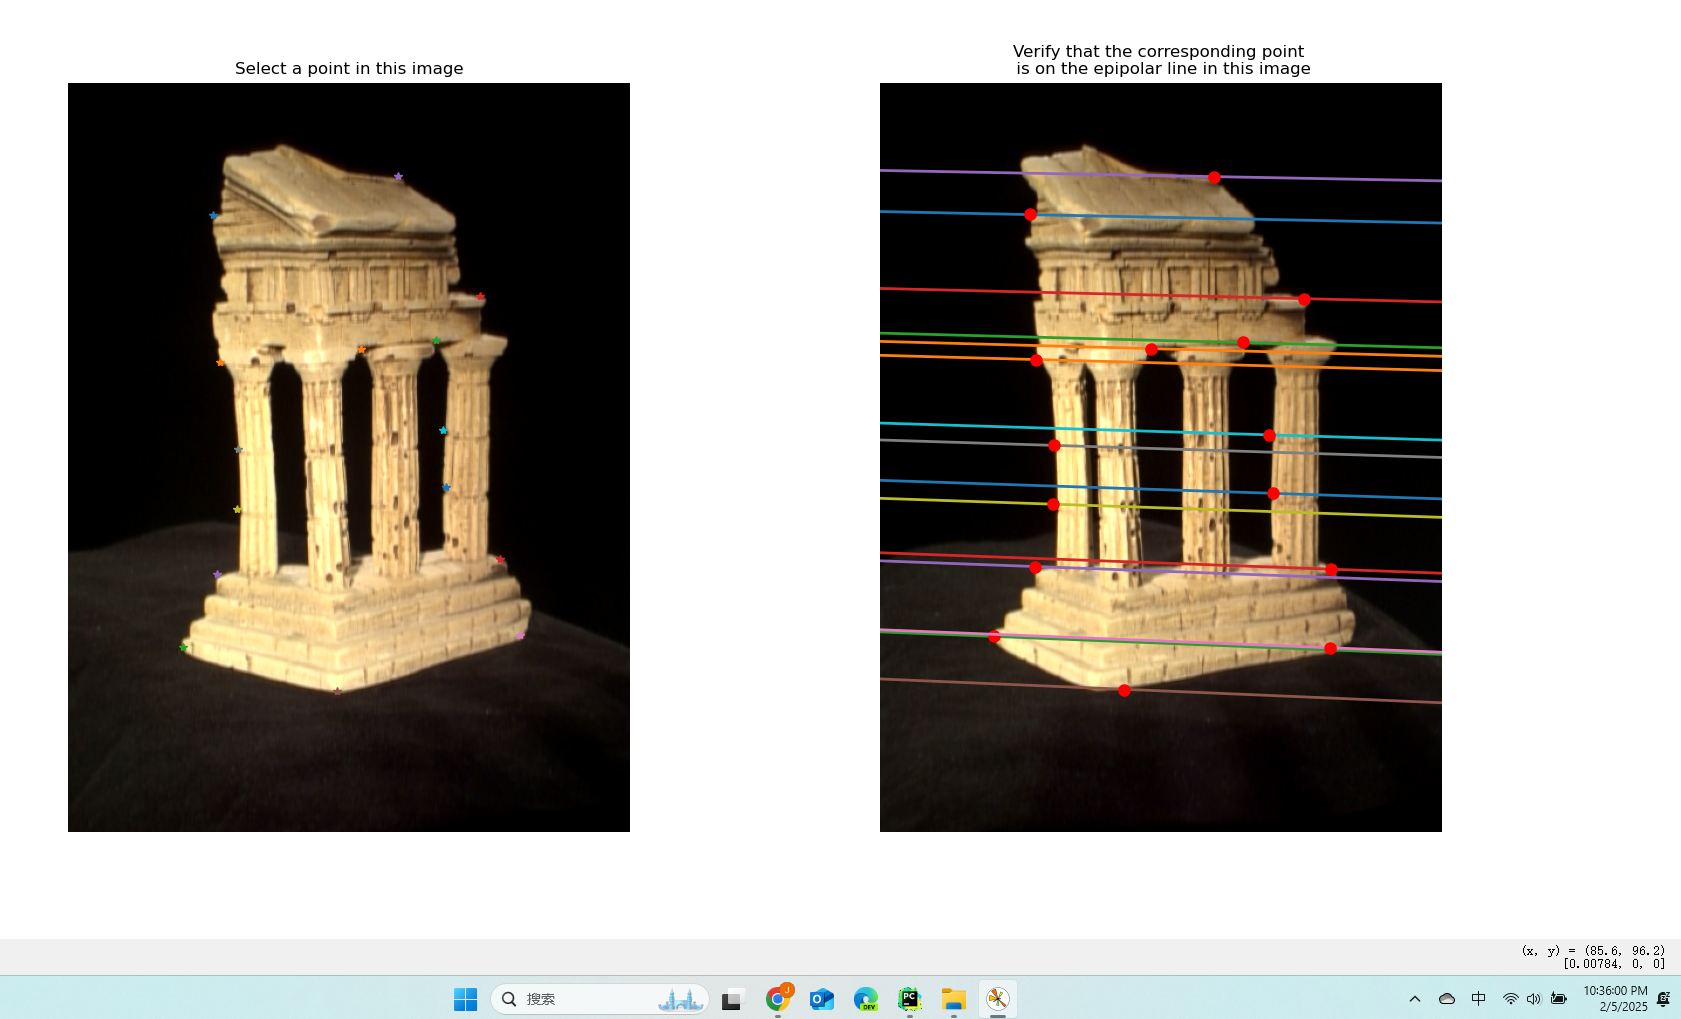
\includegraphics[width=0.66\textwidth]{media/Epiploar correspondence.png} % Replace with your image file name and extension
  \caption{Sample image for GUI output for epipolar correspondences}
  \label{fig:epipolar_corresp}
\end{figure}

\addtocounter{problemnumber}{1}
\noindent\textbf{Problem \arabic{problemnumber}}:  Compute the Essential Matrix

i. Discuss the essential matrix calculation. Briefly discuss the equation/derivation for obtaining the essential matrix from the fundamentals and the intrinsics. What does the essential matrix represent? Report your obtained essential matrix to 4 significant figures below in equation \ref{eq:essential_matrix}.

The fundamental matrix E is a special case of $F$. When the phase plane is normalized, we have $E=F$
$F$ be the fundamental matrix.
$K_1$ and $K_2$ be the $3x3$ camera intrinsic matrices for the first and second cameras, respectively. 
$E$ be the essential matrix.
$$E = K_2^T * F * K_1$$

\begin{align}
E = \begin{bmatrix}
\multicolumn{1}{c}{8.240 \times 10^{-3}} & \multicolumn{1}{c}{-1.374 \times 10^{-1}} & \multicolumn{1}{c}{-4.568 \times 10^{-2}} \\ 
\multicolumn{1}{c}{-3.035 \times 10^{-1}} & \multicolumn{1}{c}{-3.052 \times 10^{-3}} & \multicolumn{1}{c}{1.655 \times 10^{0}} \\ 
\multicolumn{1}{c}{-1.129 \times 10^{-3}}  & \multicolumn{1}{c}{-1.676 \times 10^{0}} & \multicolumn{1}{c}{-2.873 \times 10^{-3}} \\ 
\end{bmatrix}
\label{eq:essential_matrix}
\end{align}

\addtocounter{problemnumber}{1}
\noindent\textbf{Problem \arabic{problemnumber}}:  Triangulation

i. Discuss the process for determining the correct extrinsic matrix. After decomposition, how did you determine which extrinsic matrix was correct - what did you look at? If you automated this process, descibe your algorithm. Report the determined extrinsic matrix below in equation \ref{eq:extrinsic_matrix} to 4 significant figures.

\begin{align}
Ext=\begin{bmatrix}
0.0011 & 0.0012 & 0.0013 \\ 
0.0021 & 0.0022 & 0.0023 \\ 
0.0031 & 0.0032 & 0.0033 \\ 
\end{bmatrix}
\label{eq:extrinsic_matrix}
\end{align}


The process of determining the correct extrinsic matrix involves decomposing the Essential matrix \(E\) into possible rotation matrices (\(R_1, R_2\)) and a translation vector (\(t\)). Since the Essential matrix only provides relative motion up to a scale, four possible extrinsic matrices can be formed:

\[
P_2 = 
\begin{bmatrix}
R_1 & t
\end{bmatrix}, \quad
\begin{bmatrix}
R_2 & t
\end{bmatrix}, \quad
\begin{bmatrix}
R_1 & -t
\end{bmatrix}, \quad
\begin{bmatrix}
R_2 & -t
\end{bmatrix}
\]
To determine which \(P_2\) is correct, we use a point-in-front constraint. After triangulation, a 3D point \(X\) should lie in front of both cameras, meaning:
\[
X_{Z,1} > 0 \quad \text{(in front of Camera 1)}
\]
\[
X_{Z,2} > 0 \quad \text{(in front of Camera 2)}
\]

For each candidate \(P_2\), we count the number of valid 3D points that satisfy this constraint and choose the matrix that results in the highest count.

After running the algorithm, the best extrinsic matrix \(P_2\) was determined.

\hrule

ii. Discuss the setup of the SVD problem - what did the final equations you used look like to determine the $A$ matrix? Report and discuss your reprojection error to 6 significant figures in equation \ref{eq:reprojection_error_3d}. What does this error represent? What units is it in?

\begin{equation}
errror_{reprojection3d}=0.630593 \label{eq:reprojection_error_3d}
\end{equation}

Let \(\mathbf{X} = [X \; Y \; Z \; 1]^T\) be the homogeneous coordinates of a 3D point. Its projections onto two images are given by
\[
\lambda_1\,\mathbf{m}_1 = P_1\,\mathbf{X} \quad \text{and} \quad \lambda_2\,\mathbf{m}_2 = P_2\,\mathbf{X},
\]
where
\[
\mathbf{m}_1 = \begin{bmatrix} x_1 \\ y_1 \\ 1 \end{bmatrix}, \quad
\mathbf{m}_2 = \begin{bmatrix} x_2 \\ y_2 \\ 1 \end{bmatrix},
\]
and \(P_1\) and \(P_2\) are the \(3\times4\) projection matrices for camera 1 and camera 2, respectively. In our setup, the first camera is taken as the reference with
\[
P_1 = [I \mid \mathbf{0}],
\]
and \(P_2\) is obtained (via decomposition of the Essential matrix) as one of the four possible candidates of the form
\[
P_2 = [R \mid \pm t].
\]

To eliminate the unknown scale factors \(\lambda_1\) and \(\lambda_2\), we write the projection equations in their cross-product form. For the first camera, one common formulation is:
\[
\begin{aligned}
x_1\,(P_1)_{3,:}\,\mathbf{X} - (P_1)_{1,:}\,\mathbf{X} &= 0,\\[1mm]
y_1\,(P_1)_{3,:}\,\mathbf{X} - (P_1)_{2,:}\,\mathbf{X} &= 0,
\end{aligned}
\]
and similarly for the second camera:
\[
\begin{aligned}
x_2\,(P_2)_{3,:}\,\mathbf{X} - (P_2)_{1,:}\,\mathbf{X} &= 0,\\[1mm]
y_2\,(P_2)_{3,:}\,\mathbf{X} - (P_2)_{2,:}\,\mathbf{X} &= 0.
\end{aligned}
\]

Stacking these four equations yields a homogeneous linear system:
\[
A\,\mathbf{X} = \mathbf{0},
\]
where the \(4\times4\) matrix \(A\) is constructed as
\[
A = \begin{bmatrix}
x_1\,P_1(3,:) - P_1(1,:) \\[1mm]
y_1\,P_1(3,:) - P_1(2,:) \\[1mm]
x_2\,P_2(3,:) - P_2(1,:) \\[1mm]
y_2\,P_2(3,:) - P_2(2,:)
\end{bmatrix}.
\]
Here, we adopt the common notation in computer vision where \(P_1(1,:)\) denotes the first row, \(P_1(2,:)\) the second row, and \(P_1(3,:)\) the third row of \(P_1\) (i.e., using 1-indexing for clarity).

We then solve for \(\mathbf{X}\) using Singular Value Decomposition (SVD). That is, we compute
\[
A = U\,\Sigma\,V^T,
\]
and the solution is given by the last column of \(V\) (or the last row of \(V^T\)), corresponding to the smallest singular value:
\[
\mathbf{X} = V(:, end).
\]
Finally, \(\mathbf{X}\) is normalized so that its fourth component is 1

The reprojection error measures how far (in the image plane) the 3D points, when projected back through the estimated camera model, deviate from their original 2D feature locations. The reprojection error is measured in pixels

\hrule
iii. Discuss any differences between your approach and OpenCV's approach. Are the resulting reprojection errors different? What could be the source of these differences? Report and discuss the OpenCV reprojection error to 6 significant figures in equation \ref{eq:reprojection_error_ocv}. What does this error represent? What units is it in?

\begin{equation}
errror_{reprojectionOCV}=0.630593 \label{eq:reprojection_error_ocv}
\end{equation}

Custom triangulation reprojection error: $0.630593680720684$  \\
OpenCV triangulation reprojection error: $0.6305936814281153$ \\
Unit in pxiel. \\
My approach uses Direct Linear Transform (DLT) for triangulation. OpenCV’s cv2.triangulatePoints() also uses a variant of DLT.

This is a very low reprojection error. A low reprojection error means that the estimated 3D points are consistent with the original observations, given the estimated camera parameters.

\hrule
\addtocounter{problemnumber}{1}
\noindent\textbf{Problem \arabic{problemnumber}}:  Connecting the dots and visualizing the point cloud

i. Discuss the program flow you implemented for the main function - what were the steps you took to perform 3d reconstruction in general?

1. Load Data, load the corresponding 2D points from the two images, and load the camera intrinsic matrix. 

2. Using the corresponding 2D feature points, compute the fundamental matrix F

3. Using the intrinsic matrix to transform F into an essential matrix

4. By decomposing E, estimate the camera pose.

5. Use direct linear triangulation (DLT) to reconstruct the 3D point cloud.

\hrule
ii. Discuss the \texttt{visualize(point\_cloud)} function you implemented. How does it work, and what steps did you take to verify its output?

The visualize() function provides a 3D scatter plot of the triangulated point cloud using Matplotlib.visualize()

As for verification:\\
The ensured point cloud is an (N, 3) array where each row is a valid (X, Y, Z) coordinate.\\
Reviewed the structure of the point cloud to confirm it is as expected\\
Compared to OpenCV output: Plotted point\_cloud from my triangulation as well as OpenCV's version (point\_clou\_cv) to ensure consistency.\\

\hrule
iii. Replace the image in figure \ref{fig:reconstruction} with a screenshot of your 3d visualization results. Discuss your output - does it look correct to you? Are all of the points in their correct locations? Discuss the accuracy of the point locations and potential sources of error in this representation. 
It is correct.\\
But here, I emphasize, a lower error only proves that my triangulation process is consistent with the selected data, but does not mean that the real-world coordinates are necessarily accurate.\\
The back-projection error only reflects "how much the deviation is between triangulation and projection back to the original 2D point given the data and the estimated model". It can prove that the result is mathematically consistent with the input data, but it cannot absolutely guarantee "correctness in the physical and geometric sense". \\
For a particle at an extreme point, the reconstruction often has scale uncertainty. As long as it can be projected to the same 2D point, the reconstruction can be arbitrarily enlarged or reduced by a multiple, but the back-projection error is still 0\\


\hrule
\begin{figure}
  \centering
  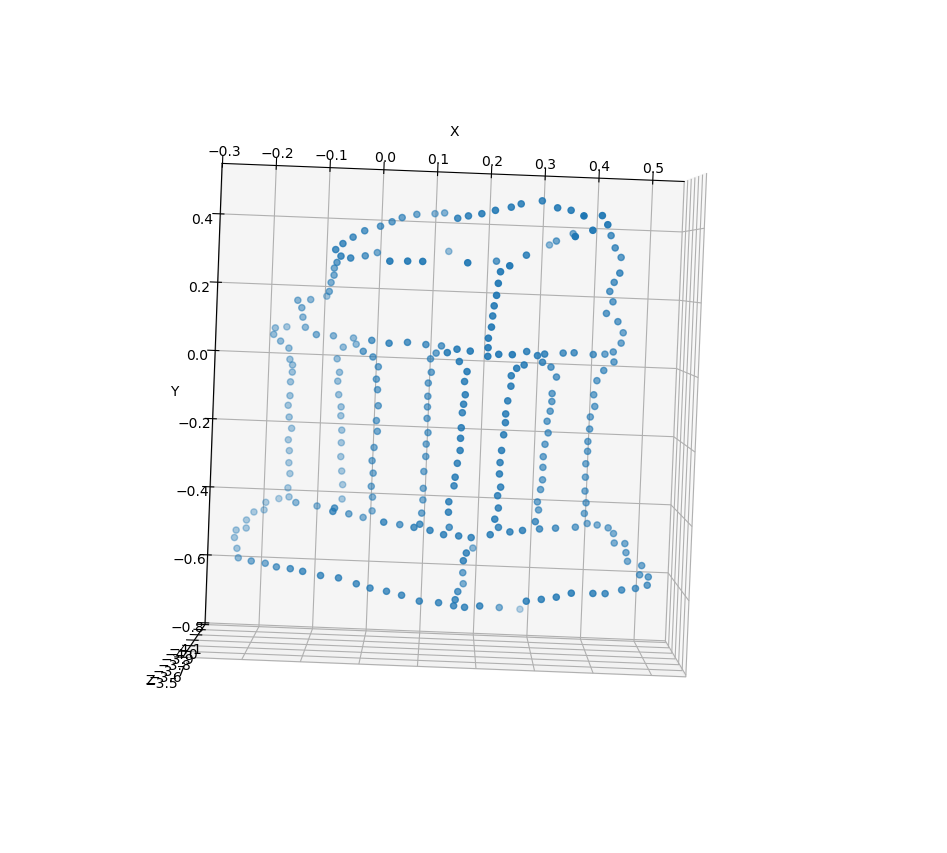
\includegraphics[width=0.66 \textwidth]{media/Reconstruction.png} % Replace with your image file name and extension
  \caption{Sparse Reconstruction}
  \label{fig:reconstruction}
\end{figure}


\addtocounter{problemnumber}{1}
\noindent\textbf{Optional Problem \arabic{problemnumber}}: Pain points and Flash cards

i. If you had any particular difficulties in the homework, or had any extra figures, experiments, etc. you would like to show off, feel free to discuss them here.



\noindent\textbf{References and Credits:}\\
Parts of this homework are from David Fouhey's EECS 442 and CMU 16-385, and from Jason Corso's ROB 498/599 classes.

\end{document}